\setlength{\columnsep}{3pt}
\begin{flushleft}
\bigskip


\begin{itemize}
	\item Hostname is the name of your computer.
	
	\item \textbf{Fully qualified domain name (FQDN)} is hostname plus the domain.
	
	\item Example of hostname, domain name and FQDN is:
	\begin{itemize}
		\item \textbf{Hostname}: server
		\item \textbf{Domain}: example.com
		\item \textbf{FQDN}: server.example.com
	\end{itemize}
	\bigskip
	\item Command to assign hostname:
	\begin{tcolorbox}[breakable,notitle,boxrule=-0pt,colback=pink,colframe=pink]
		\color{black}
		\fontdimen2\font=1em
		Syntax: hostnamectl set-hostname FQDN
		\fontdimen2\font=4pt
	\end{tcolorbox}
	\bigskip
	\item Eg:
	\begin{tcolorbox}[breakable,notitle,boxrule=-0pt,colback=black,colframe=black]
		\color{green}
		\fontdimen2\font=1em
		\# hostnamectl set-hostname server.example.com
		\fontdimen2\font=4pt
	\end{tcolorbox}

	\item Command to check hostname status:
	\begin{tcolorbox}[breakable,notitle,boxrule=-0pt,colback=pink,colframe=pink]
		\color{black}
		\fontdimen2\font=1em
		Syntax: hostnamectl status
		\fontdimen2\font=4pt
	\end{tcolorbox}
	\bigskip
	\item Eg:
	\begin{figure}[h!]
		\centering
		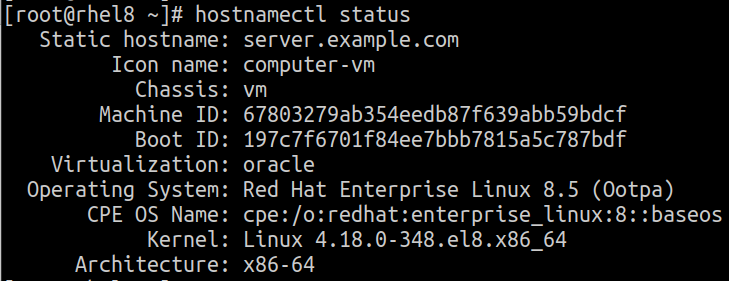
\includegraphics[scale=.35]{content/chapter14/images/hostname.png}
		\caption{Sample output}
		\label{fig:hoststatus}
	\end{figure}		

	\bigskip
	\item In RHEL 8, the hostname is stored in \textbf{/etc/hostname} file. Changes in this file will be reflected only after server reboot.
	
	

\end{itemize}



\end{flushleft}
\newpage


